\begin{IEEEbiography}[{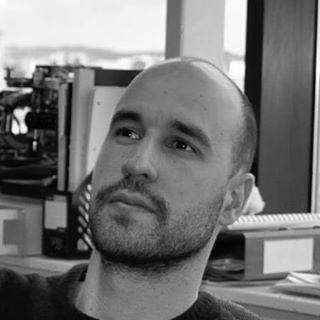
\includegraphics[width=1in,height=1.25in,clip,keepaspectratio]{images/nuno}}]{Nuno Moutinho}
Nuno Moutinho is a PhD student and researcher at the Dept. of Electrical and Computer Engineering of the Faculty of Engineering at IST, the Faculty of Engineering in the Technical University of Lisbon.

His main research interests focus on computer vision applied to robotic systems, self-calibration mechanisms for robotic platforms, visual SLAM, augmented reality and Expected Perception mechanisms. He has published works on Expected Perception, kinematic self-calibration of robotic platforms and automatic calibration of stereo systems in several international conferences. He has been participating in many national and international projects involving both academic and industrial partners. He is also the co-founder and CTO of boomApp, a computer vision startup specialized in large scale video recognition algorithms.
\end{IEEEbiography}

\begin{IEEEbiography}[{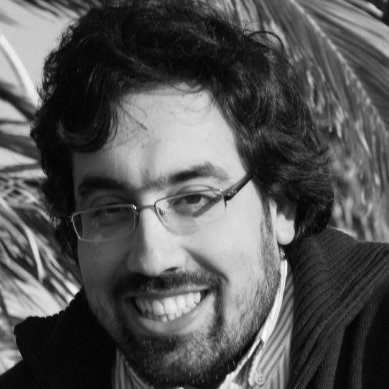
\includegraphics[width=1in,height=1.25in,clip,keepaspectratio]{images/ricardo}}]{Ricardo Ferreira}
\end{IEEEbiography}

\begin{IEEEbiography}[{
\includegraphics[width=1in,height=1.25in,clip,keepaspectratio]{images/gaspar}}]{Jose Gaspar}
\end{IEEEbiography}

\begin{IEEEbiography}[{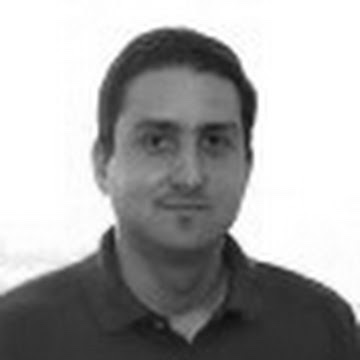
\includegraphics[width=1in,height=1.25in,clip,keepaspectratio]{images/alex}}]{Alexandre Bernardino}

Alexandre Bernardino is an Associate Professor at the Dept. of Electrical and Computer Engineering of the Faculty of Engineering at IST, the Faculty of Engineering in the Technical University of Lisbon.
He teaches on the scientific area of decision systems and control, in courses involving signal and image processing, automation and robotics, modeling and control, artificial intelligence and machine learning.

He's a senior researcher at ISR-Lisboa (the Institute for Systems and Robotics of IST), member of LARSyS (Laboratory of Robotics, Systems of Engineering and Science), and co-director of VisLab, the Computer and Robot Vision Laboratory.
His main research interests focus on the application of computer vision, cognitive science, control theory and machine learning to advanced robotic and surveillance systems.
He has published works on foveal sensors, visual attention and stereo, image feature extraction, binocular head control, image based tracking and identification, learning object affordances, sensorimotor coordination, human activity recognition, among other topics. He has been participating in many national and international projects involving both academic and industrial partners.
\end{IEEEbiography}